% Fakesection 序言之前

\RequirePackage[l2tabu, orthodox]{nag}
\RequirePackage{ifxetex}
\RequireXeTeX
\documentclass{ctexart}

%颜色
\usepackage{xcolor}

%长度
\usepackage{printlen}
\uselengthunit{mm}


%图形
\usepackage{media9}
\usepackage{pdfpages}
\usepackage{overpic}
\usepackage{graphicx}
\graphicspath{{./src/}}
\usepackage{wallpaper}
\usepackage{wrapfig}
\usepackage{pstricks}
\usepackage{smartdiagram}
\usepackage[edges]{forest}
\usepackage{pgfplots}
\usepackage{tikz}
\usetikzlibrary{shapes.geometric}
\usetikzlibrary{calc}
\usetikzlibrary{patterns}
\usetikzlibrary{arrows}
\usetikzlibrary{shapes}
\usetikzlibrary{chains}
\usetikzlibrary{mindmap}
\usetikzlibrary{graphs}
\usetikzlibrary{decorations.text}
\usetikzlibrary{arrows.meta}
\usetikzlibrary{shadows.blur}
\usetikzlibrary{shadings}
\usepackage{scsnowman}
\usepackage{tikzpeople}
\usepackage{tikzducks}
\usepackage{flowchart}
\usepackage{ean13isbn}
\usepackage{qrcode}
\usepackage{pgf-pie}
\usepackage{pgfmath}

%表格
\usepackage{tabu}
\usepackage{longtable}
\usepackage{booktabs}
\usepackage{diagbox}
\usepackage{multicol}
\usepackage{multirow}
\usepackage{makecell}
\usepackage{fancybox}
\usepackage{colortbl}
\usepackage{tcolorbox}
\tcbuselibrary{skins}
\tcbuselibrary{breakable}
\tcbuselibrary{theorems}
\tcbuselibrary{listings}
\tcbuselibrary{xparse}
\usepackage{fvextra}
\usepackage{csvsimple}
\usepackage{boxedminipage2e}

%公式
\usepackage{amsmath}
\usepackage{amsthm}
\usepackage{amsfonts}
\usepackage{amssymb}
\usepackage{amsbsy}
\usepackage{amsopn}
\usepackage{amstext}
\usepackage{mathrsfs}
\usepackage{bm}
\usepackage{textcomp}
\usepackage{latexsym}
\usepackage{exscale}
\usepackage{relsize}
%\usepackage{xymtex}
\usepackage{physics}
\usepackage{siunitx}
\usepackage{hologo}
\usepackage{cases}

%正文
\usepackage{fancyhdr}
\usepackage{geometry}
\usepackage{lastpage}
\usepackage{indentfirst}
\usepackage{setspace}
\renewcommand\arraystretch{1.5}

%非正文
\usepackage{makeidx}
\makeindex
\usepackage{epigraph}
\usepackage{varwidth}

%参考文献
\usepackage{morewrites}
\renewcommand{\thefootnote}{\fnsymbol{footnote}}
\usepackage[resetlabels]{multibib}
\newcites{sec}{参考网站}

%%链接
\usepackage
[	colorlinks = true,
linkcolor = gray,
citecolor = gray,
backref=page
]{hyperref}
\usepackage{caption}
\usepackage{subcaption}

%其它
\usepackage{atbegshi}
\usepackage{lipsum}

%文字
\usepackage{csquotes}
\usepackage{microtype}

\csname
endofdump
\endcsname

%\usepackage[notref,notcite]{showkeys}

%%代码
\usepackage{minted}
\usepackage{pygmentex}
\tcbuselibrary{minted}% 用minted排版代码
%Java %与mcode冲突
% \usepackage{lstcustom}
%Matlab %与lstcustom冲突
%\usepackage[framed,numbered,autolinebreaks,useliterate]{mcode}
\usepackage{boxie}
\makeatletter
\xdefinecolor{tcbcol@back}{rgb}{0,0,0}
\makeatother

%枚举%与beamer冲突
\usepackage{enumitem}
\setlist[enumerate, 2]
{	fullwidth,
	label = \alph*.,
	font = \textup,
	itemindent=2em
}

\usepackage{titlesec}
%\titleformat{\chapter}{\centering\Huge\bfseries}{实验\chinese{chapter}}{~}{0pt}
\titleformat{\section}{\centering\LARGE\bfseries}{\thesection~}{0pt}{}
\titleformat{\subsection}{\Large}{\chinese{subsection}、~}{0pt}{}
\titleformat{\subsubsection}{\large}{\arabic{subsubsection}.~}{0pt}{}

\newif\ifOne\Onefalse
\newif\ifTwo\Twofalse
\newif\ifThree\Threefalse
\newif\ifFour\Fourfalse

\ifnum\strcmp{\jobname}{1}=0
	\Onetrue
\fi
\ifnum\strcmp{\jobname}{2}=0
	\Twotrue
\fi
\ifnum\strcmp{\jobname}{3}=0
	\Threetrue
\fi
\ifnum\strcmp{\jobname}{4}=0
	\Fourtrue
\fi
\ifnum\strcmp{\jobname}{main}=0
	\Onetrue
	\Twotrue
	\Threetrue
	\Fourtrue
\fi

\begin{document}

% Fakesection 扉页

\begin{titlepage}
	\centering
	\begin{figure}[htpb]
		\centering
		\includegraphics[width=.8\linewidth]{NJUST.ai}
		\label{fig:NJUST}
	\end{figure}

	\vspace{20mm}

	\textbf{\heiti\zihao{1}微机原理及应用}

	\vspace{5mm}

	\textbf{\heiti\zihao{1}{综合实验报告}}

	\vspace{20mm}

	\begin{table}[htpb]
		\centering
		\zihao{3}
		\begin{tabu}to.8\linewidth{@{}X[6,r]@{}X[c]@{}X[12,l]@{}}
			\makebox[6\ccwd][s]{姓名}&:&\underline{\makebox[12\ccwd][c]{\kaishu{吴振宇}}}\\
			\makebox[6\ccwd][s]{学号}&:&\underline{\makebox[12\ccwd][c]{\kaishu{916101630117}}}\\
			\makebox[6\ccwd][s]{班级}&:&\underline{\makebox[12\ccwd][c]{\kaishu{9171040G11}}}\\
			\makebox[6\ccwd][s]{登陆号}&:&\underline{\makebox[12\ccwd][c]{029}}\\
			\makebox[6\ccwd][s]{自我评定成绩}&:&\underline{\makebox[12\ccwd][c]{A}}\\
			\makebox[6\ccwd][s]{最后成绩}&:&\underline{\makebox[12\ccwd][c]{}}\\
		\end{tabu}
	\end{table}

	\vspace{10mm}
	\zihao{3}
	\kaishu{\today}
\end{titlepage}

%页眉页脚%与book冲突
\pagestyle{fancy}
\renewcommand{\headrulewidth}{0pt}
\lhead{}
\chead{}
\rhead{}
\lfoot{\small{\leftmark}}
\cfoot{\small{第\thepage 页~共~\pageref{LastPage}~页}}
\rfoot{\small{\rightmark}}

% Fakesection 1

\ifOne
	\section{汇编语言编程与调试}%
	\label{sec:汇编语言编程与调试}

	\subsection{实验目的}%
	\label{sub:实验目的\chinese{section}}

	熟悉x86汇编开发环境,为之后的开发累实基础。

	\begin{enumerate}
		\item 搭建x86跨平台开发环境;
		\item 掌握汇编语言编程与调试。
	\end{enumerate}

	\subsection{实验设备}%
	\label{sub:实验设备\chinese{section}}

	PC机一台。

	\subsection{实验内容}%
	\label{sub:实验内容\chinese{section}}

	\subsection{实验步骤}%
	\label{sub:实验步骤\chinese{section}}

	\subsubsection{x86开发平台搭建}%
	\label{ssub:x86开发平台搭建}

	\paragraph{运行环境}%
	\label{par:运行环境}

	个人PC机是64位Win10,需要安装16位MSDOS虚拟机提供运行环境。同时后期开发也将在虚拟机中进行编译和调试。

	\winlightfile{命令提示符}{src/win10.txt}

	虚拟机选择DOSBox。往配置文件dosbox-0.74.conf写入初始化命令,可以省去每次启动时,挂载工作目录的麻烦。

	\begin{verbatim}
[autoexec]
# Lines in this section will be run at startup.
# You can put your MOUNT lines here.

mount C D:\ProgramData\MSDOS
C:
cd TC
cls
dir

	\end{verbatim}

	将DOSBox加入系统路径。启动参数设置为"DOSBox -noconsole",启动后只会出现1个窗口。不会出现DOSBox Status Window。运行信息则会写入挂载目录下的stderr.txt和stdout.txt。因为初始化命令,每次启动后会自动进入TC文件夹。将这里作为工作目录,需要使用的软件都会安装在这里。

	\begin{figure}[htpb]
		\centering
		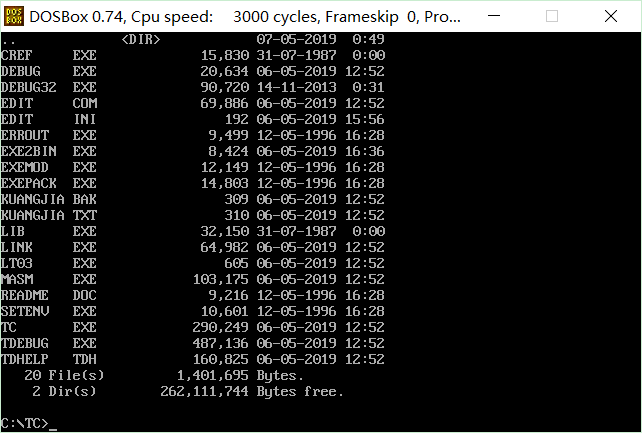
\includegraphics[width=0.8\linewidth]{DOSBox.png}
		\caption{DOSbox}
		\label{fig:DOSBox}
	\end{figure}

	\paragraph{开发环境}%
	\label{par:开发环境}

	DOSBox只提供了运行环境,能够让16位的DOS软件运行。但开发环境还需另行搭建。

	比较简单的方法是直接使用集成开发环境。常见的x86汇编集成开发环境有emu8086和masm集成开发环境。如图\ref{fig:emu8086}和\ref{fig:masm集成开发环境}。两者都自带了虚拟机提供运行环境。其中masm集成开发环境使用的运行环境就是DOSBox。

	\begin{figure}[htpb]
		\centering
		\begin{subfigure}[htpb]{.45\linewidth}
			\centering
			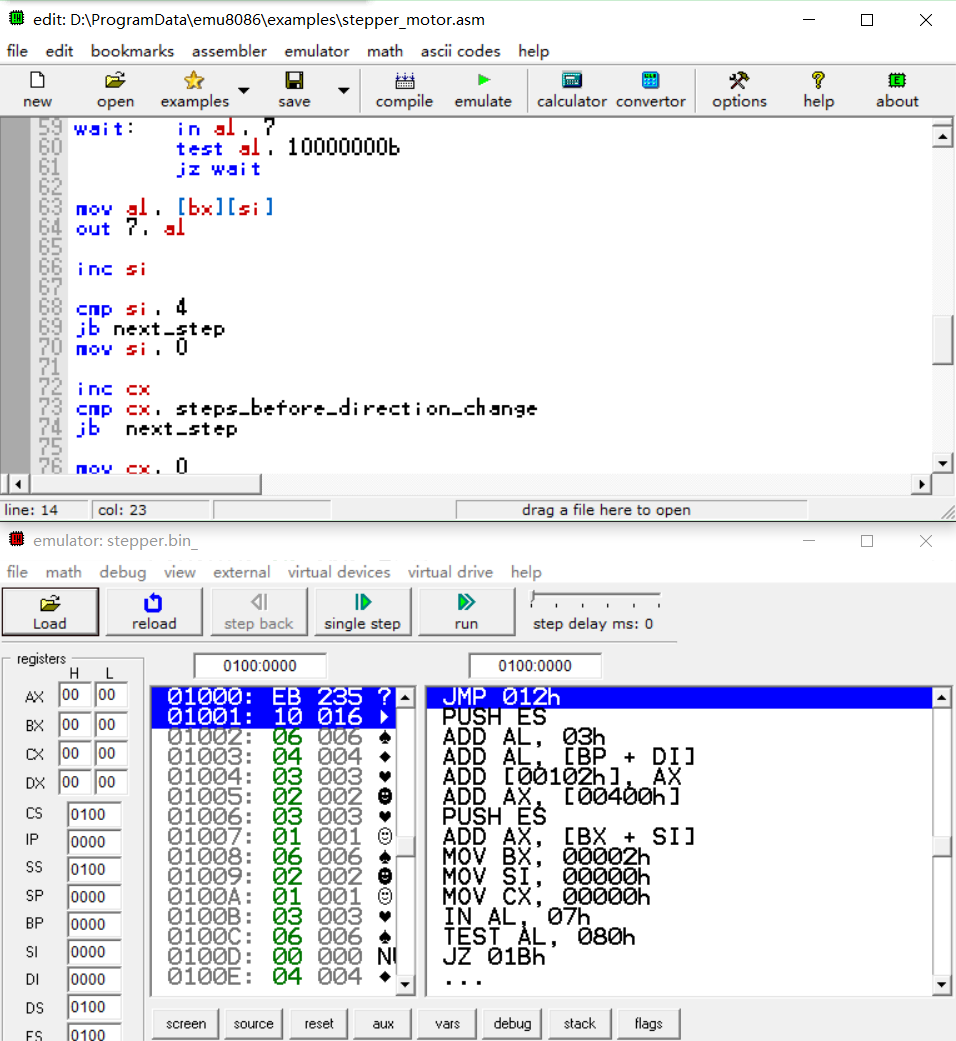
\includegraphics[width=\linewidth]{emu8086.png}
			\caption{emu8086}
			\label{fig:emu8086}
		\end{subfigure}
		\quad
		\begin{subfigure}[htpb]{.45\linewidth}
			\centering
			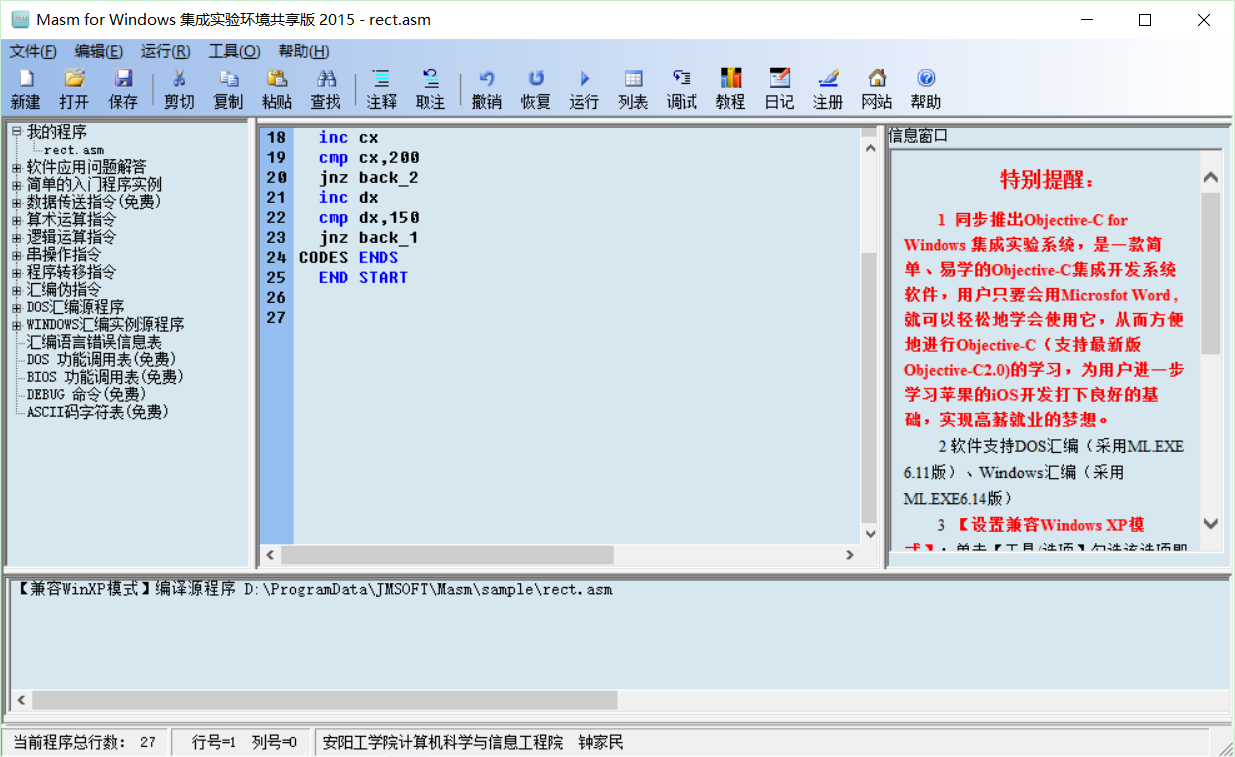
\includegraphics[width=\linewidth]{masmIDE.png}
			\caption{masm集成开发环境}
			\label{fig:masm集成开发环境}
		\end{subfigure}
		\caption{x86汇编集成开发环境}
		\label{fig:x86汇编集成开发环境}
	\end{figure}

	这些集成开发环境省去了初学者的很多麻烦,但集成化导致开发组件不方便随意更改,并不适用于真正的开发。所以考虑自己安装各种开发组件。

	一个开发环境主要包括编辑器、工具链。在工作目录里依次安装相关软件。masm.exe是x86汇编工具,link.exe是链接工具,debug.exe、debug32.exe、Tdebug.exe都是调试工具。可以在16位MSDOS中运行的编辑器有edit.exe(已停止维护和更新)、vim.exe(7.1版本之后不再支持MSDOS)和TC(同时也是1个C语言的编译器)。当然也可以在虚拟环境外用编辑器编辑后再在虚拟环境中运行。

	\begin{figure}[htpb]
		\centering
		\begin{subfigure}[htpb]{.8\linewidth}
			\centering
			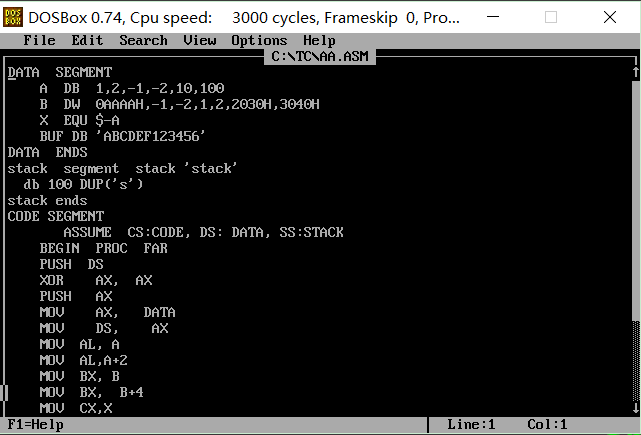
\includegraphics[width=\linewidth]{edit.png}
			\caption{edit.exe}
			\label{fig:edit.exe}
		\end{subfigure}

		\begin{subfigure}[htpb]{.8\linewidth}
			\centering
			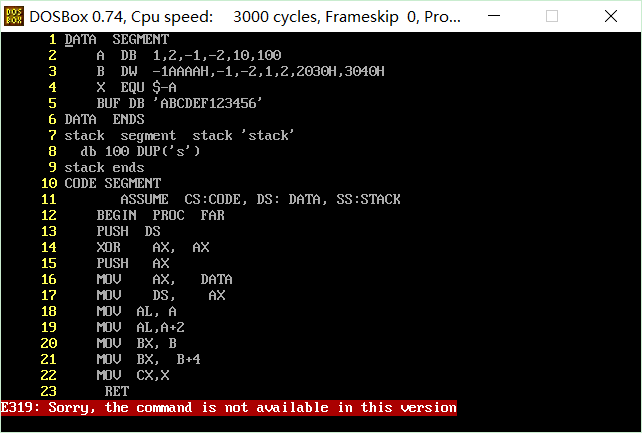
\includegraphics[width=\linewidth]{Vim71.png}
			\caption{Vim71}
			\label{fig:Vim71}
		\end{subfigure}
	\end{figure}

	\begin{figure}[htpb]
		\centering
		\begin{subfigure}[htpb]{0\linewidth}
		\end{subfigure}

		\setcounter{subfigure}{2}
		\begin{subfigure}[htpb]{.7\linewidth}
			\centering
			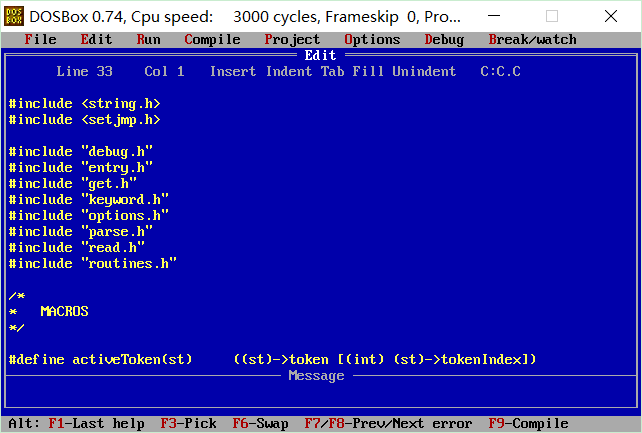
\includegraphics[width=\linewidth]{TC.png}
			\caption{TC}
			\label{fig:TC}
		\end{subfigure}
		\caption{编辑器}
		\label{fig:编辑器}
	\end{figure}

	\newpage

	\subsubsection{x86汇编开发}%
	\label{ssub:x86汇编开发}

	\paragraph{编辑代码}%
	\label{par:编辑代码}

	打开任意一种文本编辑器新建一个后缀名为asm的文件。编辑后保存就行。

	\begin{figure}[htpb]
		\centering
		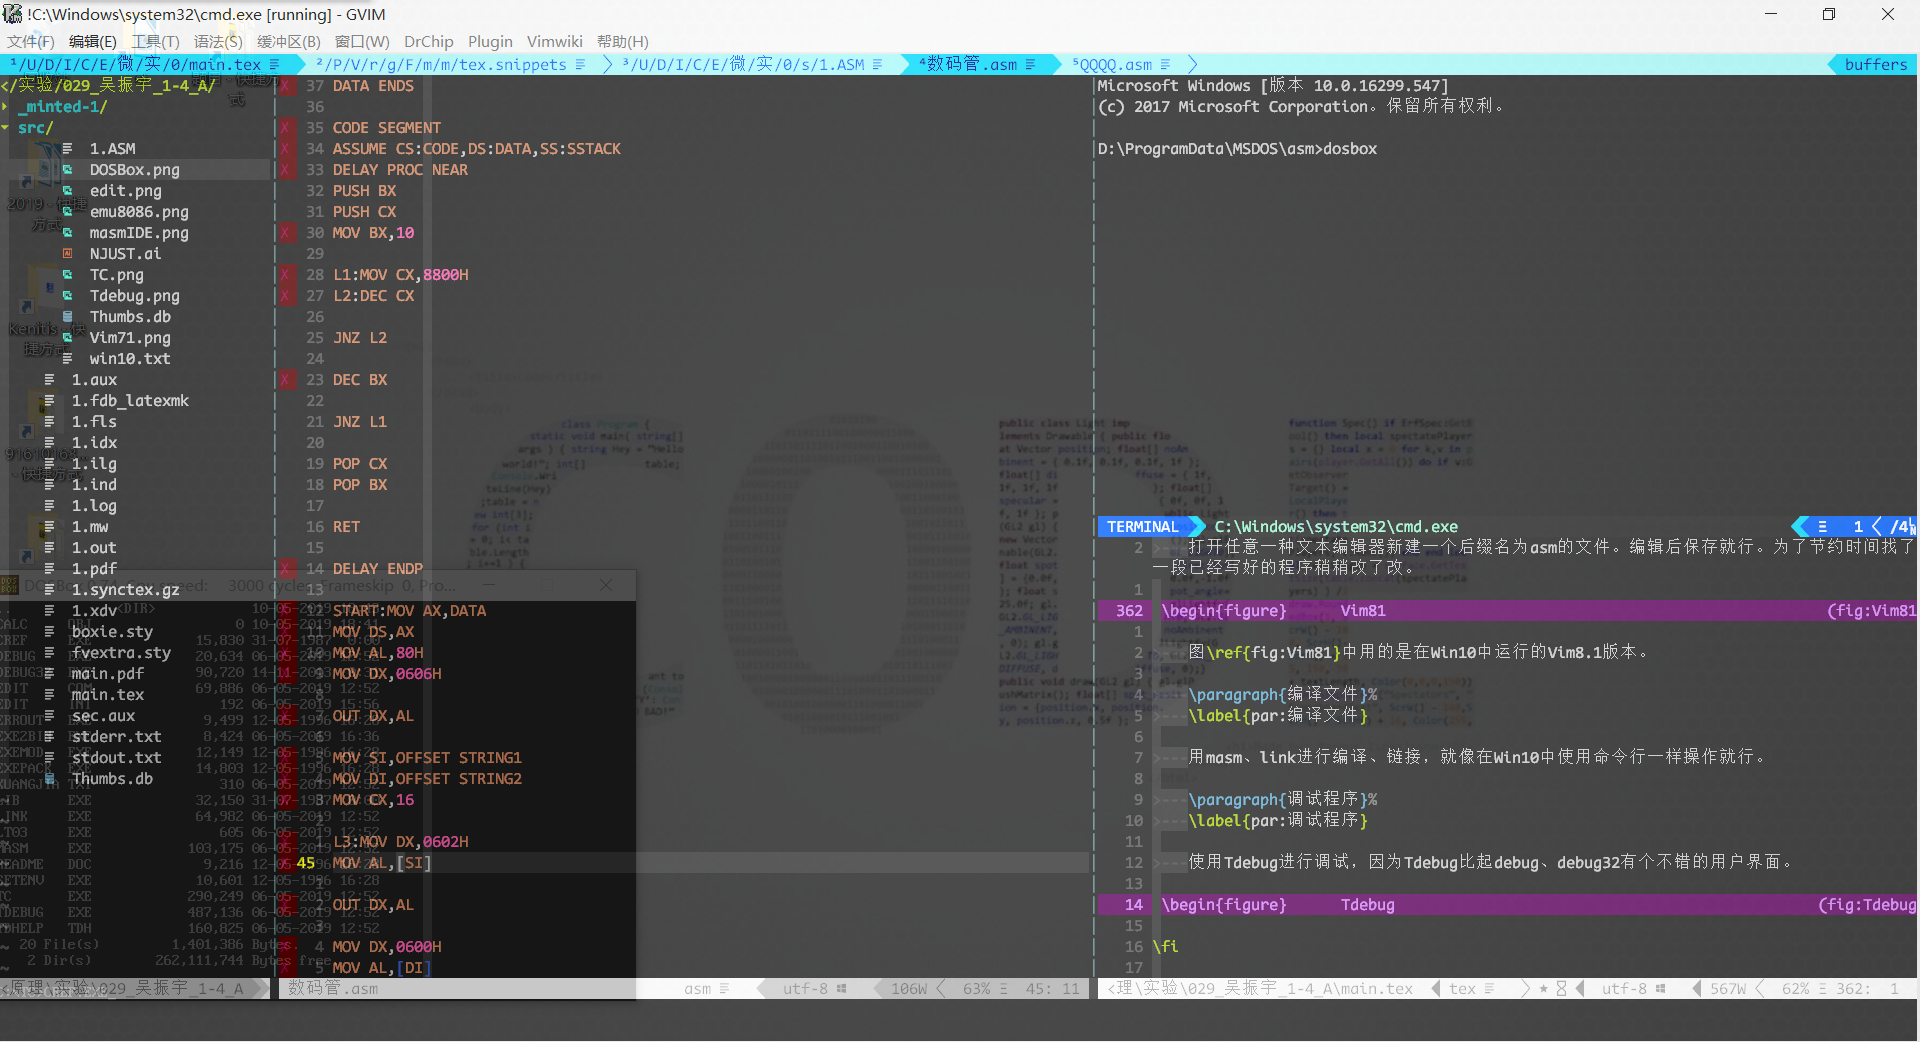
\includegraphics[width=0.6\linewidth]{Vim81}
		\caption{Vim81}
		\label{fig:Vim81}
	\end{figure}

	图\ref{fig:Vim81}中用的是在Win10中运行的Vim8.1版本。

	\paragraph{编译文件}%
	\label{par:编译文件}

	用masm、link进行编译、链接,就像在Win10中使用命令行一样操作就行。

	\paragraph{调试程序}%
	\label{par:调试程序}

	使用Tdebug进行调试,因为Tdebug比起debug、debug32有个不错的用户界面。

	\begin{figure}[htpb]
		\centering
		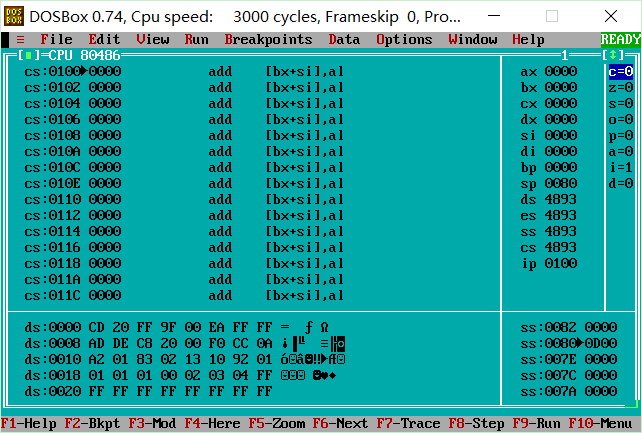
\includegraphics[width=.8\linewidth]{Tdebug.png}
		\caption{Tdebug}
		\label{fig:Tdebug}
	\end{figure}

	如图,屏幕左上、左下、右下各有3个区域,分别是指令查看窗口、数据查看窗口和堆栈查看窗口,其中指令查看窗口和数据查看窗口都分成了左边的16进制显示和右边的ASCII字符显示,而堆栈只有16进制显示。右上则有2个区域,分别是除标志位寄存器以外的寄存器和标志位,都以16进制的形式显示。按Tab能在各个窗口之间切换,按上下左右能够移动光标,按<F2>打断点,按<F7>断点调试,按<F8>单步调试,按<F9>直接运行。另外菜单栏的文件选项下面有DOS shell的选项,可以不退出Tdebug直接运行DOS shell指令。远比debug和debug32要方便。

	\langCVfile[nasm][code:1][masm]{code1.asm}{src/code1.asm}

	程序我做了注释。流程图见图\ref{fig:流程图1}。

	\begin{figure}[htpb]
		\centering
		\begin{tikzpicture}[node distance=1.5cm]
			%定义流程图具体形状
			\node (开始) [draw,terminal] {开始};
			\node (dsdx赋值) [draw,predproc,below of=开始] {ds,dx赋值};
			\node (显示字符串out1) [draw,process,below of=dsdx赋值] {显示字符串out1};
			\node (显示换行) [draw,process,below of=显示字符串out1] {显示换行};
			\node (显示字符串out2) [draw,process,below of=显示换行] {显示字符串out2};
			\node (结束) [draw,terminal, below of=显示字符串out2] {结束};

			%连接具体形状
			\draw [->,>=stealth](开始) -- (dsdx赋值);
			\draw [->,>=stealth](dsdx赋值) -- (显示字符串out1);
			\draw [->,>=stealth](显示字符串out1) -- (显示换行);
			\draw [->,>=stealth](显示换行) -- (显示字符串out2);
			\draw [->,>=stealth](显示字符串out2) -- (结束);
		\end{tikzpicture}
		\caption{流程图1}
		\label{fig:流程图1}
	\end{figure}

	\subsection{实验感悟}%
	\label{sub:实验感悟}

	倒是没有遇到什么太大的困难。倒是软件下载挺烦的。不过工欲善其事,必先利其器。一个好的编辑器能大大减少编辑代码过程中出错的可能,一个好的调试工具也能方便用户快速定位到代码有问题的地方。像那种界面简陋、操作不便的软件,在实际开发中其实是根本不会有人使用的,只有给新手展示的用途和相关发展史的意义罢了。虽然比别人浪费了更多的时间,但当最后看到一个真正的开发环境被建立起来的时候,我觉得还是挺值得的。

\fi

% Fakesection 2

\ifTwo

	\section{8259中断显示Hello}%
	\label{sec:8259中断显示Hello}

	\subsection{实验目的}%
	\label{sub:实验目的\chinese{section}}

	\begin{enumerate}
		\item 掌握8259基本原理;
		\item 掌握硬中断及软中断的中断程序编写、装载及调用方法;
		\item 学习DEBUG调试程序的使用方法。
	\end{enumerate}

	\subsection{实验准备}%
	\label{sub:实验准备}

	\begin{enumerate}
		\item 复习教材《微机接口技术及应用》有关8259编程内容。
		\item 参考\enquote{汇编语言编程设计}有关书籍,预习DEBUG调试程序的使用方法。
	\end{enumerate}

	\subsection{实验内容}%
	\label{sub:实验内容}

	\begin{enumerate}
		\item 用EDIT进行文件编辑,文件名为Interrupt.ASM;
		\item 程序汇编,显示WarringErrors和SevereErrors信息,若无错则可进行链接,若有错用EDIT修改源程序后再汇编直至无错误提示通过汇编为止。;
		\item 程序链接,查子目录中文件,可见SOUND.OBJ、COMMU.LST、SOUND.EXE文件已存在;
		\item 运行程序,从键盘输入发送内容,以自测方式,接受发送内容并显示在屏幕上。
	\end{enumerate}

	\langCVfile[nasm][code:2][masm]{code2.asm}{src/code2.asm}

	程序做了修改,原有的程序有些瑕疵,修改了8259的中断屏蔽标志位寄存器后没有复原。但不影响使用。修正了原始程序的错误,把25H 改成了35H。将程序流程图见图\ref{fig:流程图2}。

	\begin{figure}[htpb]
		\centering
		\begin{subfigure}[htpb]{.45\linewidth}
			\centering
			\begin{tikzpicture}[node distance=1.2cm]
				%定义流程图具体形状%不要使用',',否则会报错
				\node (开始) [draw, terminal] {开始};
				\node (取原中断地址) [draw, predproc, below of= 开始] {取原中断地址};
				\node (保护原中断地址) [draw, storage, below of= 取原中断地址] {保护原中断地址};
				\node (设新中断地址) [draw, predproc, below of= 保护原中断地址] {设新中断地址};
				\node (修改8259) [draw, predproc, below of= 设新中断地址] {修改8259};
				\node (中断使能) [draw, process, below of= 修改8259] {中断使能};
				\node (等待中断) [draw, decision, below of= 中断使能, yshift=-1cm] {等待中断};
				\node (中断) [draw, process, right of= 等待中断,xshift=2cm] {中断};
				\node (恢复原中断地址) [draw, predproc, below of= 等待中断,yshift=-1cm] {恢复原中断地址};
				\node (恢复8259) [draw, predproc, below of= 恢复原中断地址] {恢复8259};
				\node (结束) [draw, terminal, below of= 恢复8259] {结束};
				%连接具体形状
				\draw [->,>=stealth](开始) -- (取原中断地址);
				\draw [->,>=stealth](取原中断地址) -- (保护原中断地址);
				\draw [->,>=stealth](保护原中断地址) -- (设新中断地址);
				\draw [->,>=stealth](设新中断地址) -- (修改8259);
				\draw [->,>=stealth](修改8259) -- (中断使能);
				\draw [->,>=stealth](中断使能) -- (等待中断);
				\path(中断使能)--(等待中断)coordinate[pos=0.5](temp);
				\draw [->,>=stealth](等待中断) -- ++(2,0)node[anchor=south]{是}-- (中断);
				\draw [->,>=stealth](中断) |- (temp);
				\draw [->,>=stealth](等待中断) -- ++(0,-1.5)node[anchor=west]{否}-- (恢复原中断地址);
				\draw [->,>=stealth](恢复原中断地址) -- (恢复8259);
				\draw [->,>=stealth](恢复8259) -- (结束);
			\end{tikzpicture}
			\caption{流程图2主程序}
			\label{fig:流程图2主程序}
		\end{subfigure}
		\quad
		\begin{subfigure}[htpb]{.45\linewidth}
			\centering
			\begin{tikzpicture}[scale=1, transform shape]
				\node (进入中断) [draw, terminal] {进入中断};
				\node (中断禁止) [draw, process, below of= 进入中断] {中断禁止};
				\node (判断count 是否为0) [draw, decision, below of= 中断禁止,yshift=-2cm] {判断count 是否为0};
				\node (count--) [draw, process, right of= 判断count 是否为0, xshift=4cm] {count$ -- $};
				\node (输出字符串) [draw, predproc, below of= 判断count 是否为0, yshift=-2.5cm] {输出字符串};
				\node (count18) [draw, predproc, below of= 输出字符串] {count=18};
				\node (退出中断) [draw, terminal, below of= count18] {退出中断};
				\draw [->,>=stealth](进入中断) -- (中断禁止);
				\draw [->,>=stealth](中断禁止) -- (判断count 是否为0);
				\draw [->,>=stealth](判断count 是否为0) -- ($(判断count 是否为0) + (3,0)$ )node[anchor=south] {否}-- (count--);
				\draw [->,>=stealth](判断count 是否为0) -- ($(判断count 是否为0) + (0,-2.5)$ )node[anchor=west] {是}-- (输出字符串);
				\draw [->,>=stealth](输出字符串) --(count18);
				\draw [->,>=stealth](count18)--(退出中断);
				\path(count18)--(退出中断)coordinate[pos=.5](temp);
				\draw [->,>=stealth](count--) |- (temp);
			\end{tikzpicture}
			\caption{流程图2中断子程序}
			\label{fig:流程图2中断子程序}
		\end{subfigure}
		\caption{流程图2}
		\label{fig:流程图2}
	\end{figure}

	\subsection{实验感悟}%
	\label{sub:实验感悟}

	这次实验比上次的实验稍稍难了一点,但仍然可以读懂程序的逻辑。在开发环境的搭建上我将汇编、链接、运行、调试的命令行指令都和编辑器的快捷键做了绑定,可以不用手动打开DOSBox 输入指令,只需要敲击快捷键就可以直接自动汇编、链接、运行、调试,更加方便了。同时加载了masm 的语法高亮插件,在Github上找了1个asm的缩进插件,稍作了点修改,加上代码块补全,可以说是一个专业的IDE 也不为过了。

\fi

% Fakesection 3

\ifThree

	\section{中断控制器接口编程}%
	\label{sec:中断控制器接口编程}

	\subsection{实验目的}%
	\label{sub:实验目的\chinese{section}}

	\begin{enumerate}
		\item 掌握8259、8255编程方法。
		\item 学习DEBUG调试程序的使用方法。
	\end{enumerate}

	\subsection{实验准备}%
	\label{sub:实验准备}

	\begin{enumerate}
		\item 复习教材《微机接口技术及应用》有关8259编程内容。
		\item 参考\enquote{汇编语言编程设计}有关书籍,预习DEBUG调试程序的使用方法。
	\end{enumerate}

	\subsection{实验内容}%
	\label{sub:实验内容}

	\begin{enumerate}
		\item 用EDIT进行文件编辑,文件名为Interrupt.ASM;
		\item 程序汇编,显示WarringErrors和SevereErrors信息,若无错则可进行链接,若有错用EDIT修改源程序后再汇编直至无错误提示通过汇编为止。;
		\item 程序链接,查子目录中文件,可见SOUND.OBJ、COMMU.LST、SOUND.EXE文件已存在;
		\item 运行程序,从键盘输入发送内容,以自测方式,接受发送内容并显示在屏幕上。
	\end{enumerate}

	\langCVfile[nasm][code:3][masm]{code3.asm}{src/code3.asm}

	\begin{figure}[htpb]
		\centering
		\begin{subfigure}[htpb]{.45\linewidth}
			\centering
			\begin{tikzpicture}[node distance=1.2cm]
				%定义流程图具体形状%不要使用',',否则会报错
				\node (开始) [draw, terminal] {开始};
				\node (取原中断地址) [draw, predproc, below of= 开始] {取原中断地址};
				\node (保护原中断地址) [draw, storage, below of= 取原中断地址] {保护原中断地址};
				\node (设新中断地址) [draw, predproc, below of= 保护原中断地址] {设新中断地址};
				\node (修改8259) [draw, predproc, below of= 设新中断地址] {修改8259};
				\node (中断使能) [draw, process, below of= 修改8259] {中断使能};
				\node (等待中断) [draw, decision, below of= 中断使能, yshift=-1cm] {等待中断};
				\node (中断) [draw, process, right of= 等待中断,xshift=2cm] {中断};
				\node (恢复原中断地址) [draw, predproc, below of= 等待中断,yshift=-1cm] {恢复原中断地址};
				\node (恢复8259) [draw, predproc, below of= 恢复原中断地址] {恢复8259};
				\node (结束) [draw, terminal, below of= 恢复8259] {结束};
				%连接具体形状
				\draw [->,>=stealth](开始) -- (取原中断地址);
				\draw [->,>=stealth](取原中断地址) -- (保护原中断地址);
				\draw [->,>=stealth](保护原中断地址) -- (设新中断地址);
				\draw [->,>=stealth](设新中断地址) -- (修改8259);
				\draw [->,>=stealth](修改8259) -- (中断使能);
				\draw [->,>=stealth](中断使能) -- (等待中断);
				\path(中断使能)--(等待中断)coordinate[pos=0.5](temp);
				\draw [->,>=stealth](等待中断) -- ++(2,0)node[anchor=south]{是}-- (中断);
				\draw [->,>=stealth](中断) |- (temp);
				\draw [->,>=stealth](等待中断) -- ++(0,-1.5)node[anchor=west]{否}-- (恢复原中断地址);
				\draw [->,>=stealth](恢复原中断地址) -- (恢复8259);
				\draw [->,>=stealth](恢复8259) -- (结束);
			\end{tikzpicture}
			\caption{流程图3主程序}
			\label{fig:流程图3主程序}
		\end{subfigure}
		\quad
		\begin{subfigure}[htpb]{.45\linewidth}
			\centering
			\begin{tikzpicture}[scale=1, transform shape]
				\node (进入中断) [draw, terminal] {进入中断};
				\node (中断使能) [draw, process, below of= 进入中断] {中断使能};
				\node (获取键盘扫描码) [draw, predproc, below of= 中断使能] {获取键盘扫描码};
				\node (禁止读键盘扫描码) [draw, process, below of= 获取键盘扫描码] {禁止读键盘扫描码};
				\node (清除键盘缓冲区) [draw, process, below of= 禁止读键盘扫描码] {清除键盘缓冲区};
				\node (使能读键盘扫描码) [draw, process, below of= 清除键盘缓冲区] {使能读键盘扫描码};
				\node (判断键盘扫描码是否为通码) [draw, decision, below of= 使能读键盘扫描码,yshift=-2cm,align=center] {判断键盘扫描码\\是否为通码};
				\node (count++) [draw, process, below of= 判断键盘扫描码是否为通码, yshift=-2cm] {count++};
				\node (取出键盘扫描码高4位) [draw, process, below of= count++] {取出键盘扫描码高4位};
				\node (输出第一个字符) [draw, predproc, below of= 取出键盘扫描码高4位] {输出第一个字符};
				\node (取出键盘扫描码低4位) [draw, process, below of= 输出第一个字符] {取出键盘扫描码低4位};
				\node (输出第二个字符) [draw, predproc, below of= 取出键盘扫描码低4位] {输出第二个字符};
				\node (输出逗号) [draw, predproc, below of= 输出第二个字符] {输出逗号};
				\node (通过控制字发送中断结束信号) [draw, process, below of= 输出逗号] {通过控制字发送中断结束信号};
				\node (退出中断) [draw, terminal, below of= 通过控制字发送中断结束信号] {退出中断};
				\draw [->,>=stealth](进入中断) -- (中断使能);
				\draw [->,>=stealth](中断使能) -- (获取键盘扫描码);
				\draw [->,>=stealth](获取键盘扫描码) -- (禁止读键盘扫描码);
				\draw [->,>=stealth](禁止读键盘扫描码) -- (清除键盘缓冲区);
				\draw [->,>=stealth](清除键盘缓冲区) -- (使能读键盘扫描码);
				\draw [->,>=stealth](使能读键盘扫描码) -- (判断键盘扫描码是否为通码);
				\path(输出逗号)--(通过控制字发送中断结束信号)coordinate[pos=.5](temp);
				\draw [->,>=stealth](判断键盘扫描码是否为通码) -- ($(判断键盘扫描码是否为通码) + (3,0)$ )node[anchor=south] {否} --($(判断键盘扫描码是否为通码) + (4,0)$ ) |- (temp);
				\draw [->,>=stealth](判断键盘扫描码是否为通码) -- ($(判断键盘扫描码是否为通码) + (0,-2.5)$ )node[anchor=west] {是}-- (count++);
				\draw [->,>=stealth](count++) --(取出键盘扫描码高4位);
				\draw [->,>=stealth](取出键盘扫描码高4位) --(输出第一个字符);
				\draw [->,>=stealth](输出第一个字符) --(取出键盘扫描码低4位);
				\draw [->,>=stealth](取出键盘扫描码低4位) --(输出第二个字符);
				\draw [->,>=stealth](输出第二个字符) --(输出逗号);
				\draw [->,>=stealth](输出逗号)--(通过控制字发送中断结束信号);
				\draw [->,>=stealth](通过控制字发送中断结束信号)--(退出中断);
			\end{tikzpicture}
			\caption{流程图3中断子程序}
			\label{fig:流程图3中断子程序}
		\end{subfigure}
		\caption{流程图3}
		\label{fig:流程图3}
	\end{figure}

	\subsection{实验感悟}%
	\label{sub:实验感悟}

	这次实验比之前更难。我事先下载masm 的参考手册,上面有完整的x86 架构的中断大全、宏汇编语言的汇编指令和伪指令,又在网上找到了x86 架构的端口大全。非常意外的发现实验提供的键盘中断例程是从这份资料上的1个例程改的,改动也就是删掉了一些注释。所以也没有那么难了。

\fi

% Fakesection 4

\ifFour

	\section{异步串行通信接口编程}%
	\label{sec:异步串行通信接口编程}

	\subsection{实验目的}%
	\label{sub:实验目的\chinese{section}}

	\begin{enumerate}
		\item 掌握8250编程方法;
		\item 学习DEBUG调试程序的使用方法。
	\end{enumerate}

	\subsection{实验准备}%
	\label{sub:实验准备}

	\begin{enumerate}
		\item 复习教材《微机接口技术及应用》有关8250编程内容。
		\item 参考\enquote{汇编语言编程设计}有关书籍,预习DEBUG调试程序的使用方法。
	\end{enumerate}

	\subsection{实验内容}%
	\label{sub:实验内容}

	\begin{enumerate}
		\item 用EDIT进行文件编辑,文件名为Interrupt.ASM;
		\item 程序汇编,显示WarringErrors和SevereErrors信息,若无错则可进行链接,若有错用EDIT修改源程序后再汇编直至无错误提示通过汇编为止。;
		\item 程序链接,查子目录中文件,可见SOUND.OBJ、COMMU.LST、SOUND.EXE文件已存在;
		\item 运行程序,从键盘输入发送内容,以自测方式,接受发送内容并显示在屏幕上。
	\end{enumerate}

	\langCVfile[nasm][code:4][masm]{code4.asm}{src/code4.asm}

	\begin{figure}[htpb]
		\centering
		\begin{tikzpicture}[node distance=1.2cm]
			%定义流程图具体形状%不要使用',',否则会报错
			\node (开始) [draw, terminal] {开始};
			\node (允许写除数寄存器) [draw, align=center, process, below of= 开始] {允许写除数寄存器};
			\node (写分频系数) [draw, align=center, process, below of= 允许写除数寄存器] {写分频系数};
			\node (写报文格式) [draw, align=center, process, below of= 写分频系数] {写报文格式};
			\node (写自检模式、准备就绪) [draw, align=center, process, below of= 写报文格式] {写自检模式、准备就绪};
			\node (中断使能) [draw, align=center, process, below of= 写自检模式、准备就绪] {中断使能};
			\node (检查通信线路寄存器) [draw, align=center, decision, below of= 中断使能,yshift=-1cm] {检查\\通信线路\\寄存器};
			\path(中断使能)--(检查通信线路寄存器)coordinate[pos=.5](temp);
			\node (异常处理) [draw, align=center, process, left of= 检查通信线路寄存器,xshift=-2cm] {异常处理};
			\node (发送数据) [draw, align=center, process, right of= 检查通信线路寄存器,xshift=2cm] {发送数据};
			\node (查询键盘缓冲区) [draw, align=center, decision, below of= 检查通信线路寄存器,yshift=-2cm] {查询键盘\\缓冲区};
			\node (是否有键按下) [draw, align=center, decision, below of= 查询键盘缓冲区,yshift=-2cm] {等待\\有键\\按下};
			\node (将键盘输入发送到8259) [draw, align=center, process, below of= 是否有键按下,yshift=-1cm] {将键盘输入发送到8259};
			%连接具体形状
			\draw [->,>=stealth](开始) -- (允许写除数寄存器);
			\draw [->,>=stealth](允许写除数寄存器) -- (写分频系数);
			\draw [->,>=stealth](写分频系数) -- (写报文格式);
			\draw [->,>=stealth](写报文格式) -- (写自检模式、准备就绪);
			\draw [->,>=stealth](写自检模式、准备就绪) -- (中断使能);
			\draw [->,>=stealth](中断使能) -- (检查通信线路寄存器);
			\draw [->,>=stealth](检查通信线路寄存器) -- ++(0,-1.8)node[anchor=west] {其它}-- (查询键盘缓冲区);
			\draw [->,>=stealth](查询键盘缓冲区) -- ++(0,-1.5)node[anchor=east] {无缓冲}-- (是否有键按下);
			\draw [->,>=stealth](是否有键按下) -- ++(0,-1.5)node[anchor=west] {是}--  (将键盘输入发送到8259);
			\draw [->,>=stealth](检查通信线路寄存器) -- ++(1.8,0)node[anchor=south] {有数据}-- (发送数据);
			\draw [->,>=stealth](检查通信线路寄存器) -- ++(-1.8,0)node[anchor=south] {有异常}|- (异常处理);
			\draw [->,>=stealth](异常处理) |- (temp);
			\draw [->,>=stealth](发送数据) |- (temp);
			\draw [->,>=stealth](查询键盘缓冲区) -- ++(6,0)node[anchor=west] {有缓冲}|- (temp);
			\path(查询键盘缓冲区)--(是否有键按下)coordinate[pos=.5](查询键盘缓冲区是否有键按下);
			\draw [->,>=stealth](是否有键按下) -- ++(4,0)node[anchor=west] {无}|- (查询键盘缓冲区是否有键按下);
		\end{tikzpicture}
		\caption{流程图4}
		\label{fig:流程图4}
	\end{figure}

	\newpage

	\subsection{实验感悟}%
	\label{sub:实验感悟}

	这是最后一次实验了。回顾这四节课,我学会了宏汇编语言的基本语法,搭建了宏汇编语言的开发环境,掌握了8086、8259、8255、8250四种芯片的使用方法。受益匪浅。

\fi

\end{document}
\section{数码转换程序实验}%
\label{sec:数码转换程序实验}
\subsection{实验目的}%
\label{sub:实验目的\chinese{section}}
\begin{enumerate}
	\item 掌握不同进制数及编码相互转换的程序设计方法,加深对数制转换的理解:
	\item 熟悉程序调试的方法。
\end{enumerate}
\subsection{实验设备}%
\label{sub:实验设备\chinese{section}}
PC机一台、TD-PITE实验装置或TD-PITC实验装置一套。
\subsection{实验内容}%
\label{sub:实验内容\chinese{section}}
计算机输入设备输入的信息一般是由ASCII码或BCD码表示的数据或字符,CPU一般均用二进制数进行计算或其他信息处理,处理结果的输出又必须依照外设的要求变为ASCII码、BCD码或七段显示码等。因此,在应用软件中,各类数制的转换和代码的转换是必不可少的。
\subsubsection{将ASCII码表示的十进制数转换为二进制数}%
\label{ssub:将ASCII码表示的十进制数转换为二进制数}
十进制数可以表示为:Dn×10n+Dn-1×10n-1+…+D0×100=Di×10i 其中Di代表十进制数1、2、3…9、0。
上式可以转换为:ΣDi×10i=((…(Dn×10+Dn-1)×10)+Dn-2)×10+…+D1)×10+D0
由上式可归纳十进制数转换为二进制的方法:从十进制数的最高位Dn开始作乘10加次位的操作,依次类推,则可求出二进制数结果。

图2.3.2 十进制ASCII转换为二进制数参考流程

本实验要求将缓冲区中的一个五位十进制数32760的ASCII码转换成二进制数,并将转换结果按位显示在屏幕上。转换过程的参考流程如图2.3.2所示。
\subsubsection{将十进制数的ASCII码转换为BCD码}%
\label{ssub:将十进制数的ASCII码转换为BCD码}
本实验要求将一个五位十进制数的ASCⅡ码存放在数据区中,转换为BCD码并将转换结果按位存放在另一内存单元中 。若输入的不是十进制数的ASCⅡ码,则输出FF。提示:一字节ASCⅡ码取其低四位即变为BCD码。转换部分的实验流程参见图2.3.3。
\subsubsection{将十六位二进制数转换为十进制数的ASCII码}%
\label{ssub:将十六位二进制数转换为十进制数的ASCII码}
十六位二进制数的值域为0-65535,最大可转换为五位十进制数。五位十进制数可表示为:ND=D4×104+D3×103+D2×102+D1×10+D0 因此,将十六位二进制数转换为五位ASCⅡ码表示的十进制数,就是求D1-D4,并将它们转化为ASCⅡ码。
本实验要求将缓冲区中存放的000CH的ASCII码转换成十进制数,并将转换结果显示在屏幕上。转换部分的实验流程参见图2.3.4。
\subsection{实验步骤}%
\label{sub:实验步骤\chinese{section}}

\subsection{程序清单}%
\label{sub:程序清单\chinese{section}}
\lstinputlisting[language={[x86masm]Assembler}]{src/1.asm}
\section{循环程序设计实验}%
\label{sec:循环程序设计实验}
\subsection{实验目的}%
\label{sub:实验目的\chinese{section}}
\begin{enumerate}
	\item 加深对循环结构的理解;
	\item 掌握循环结构程序设计的方法以及调试方法。
\end{enumerate}
\subsection{实验设备}%
\label{sub:实验设备\chinese{section}}
PC机一台、TD-PITE实验装置或TD-PITC实验装置一套。
\subsection{实验内容}%
\label{sub:实验内容\chinese{section}}
从键盘输入一个数N,计算N!,结果(16进制)显示在屏幕上。
\subsection{实验步骤}%
\label{sub:实验步骤\chinese{section}}

\subsection{程序清单}%
\label{sub:程序清单\chinese{section}}
\lstinputlisting[language={[x86masm]Assembler}]{src/1.asm}
\subsection{程序清单}%
\label{sub:程序清单\chinese{section}}
\lstinputlisting[language={[x86masm]Assembler}]{src/1.asm}
\section{子程序设计实验}%
\label{sec:子程序设计实验}
\subsection{实验目的}%
\label{sub:实验目的\chinese{section}}
\begin{enumerate}
	\item 学习子程序的定义和调用方法;
	\item 掌握子程序、子程序的嵌套、递归子程序的结构;
	\item 掌握子程序的程序设计及调试方法。
\end{enumerate}
\subsection{实验设备}%
\label{sub:实验设备\chinese{section}}
PC机一台、TD-PITE实验装置或TD-PITC实验装置一套。
\subsection{实验内容}%
\label{sub:实验内容\chinese{section}}
将数据段中定义的十个两位16进制无符号数按从大到小的顺序排列,并依次显示在屏幕上,中间用空格分隔
\subsection{实验步骤}%
\label{sub:实验步骤\chinese{section}}

\subsection{程序清单}%
\label{sub:程序清单\chinese{section}}
\lstinputlisting[language={[x86masm]Assembler}]{src/1.asm}
\section{静态存储器扩展实验}%
\label{sec:静态存储器扩展实验}
\subsection{实验目的}%
\label{sub:实验目的\chinese{section}}
\begin{enumerate}
	\item 了解存储器扩展的方法和存储器的读/写;
	\item 掌握 CPU 对 16 位存储器的访问方法。
\end{enumerate}
\subsection{实验设备}%
\label{sub:实验设备\chinese{section}}
PC机一台、TD-PITE实验装置或TD-PITC实验装置一套。
\subsection{实验内容}%
\label{sub:实验内容\chinese{section}}
编写实验程序,将0010H~001FH共16个数写入SRAM的从8000H:0000H起始的一段空间中,然后通过系统命令查看该存储空间,检测写入数据是否正确。
\subsection{实验步骤}%
\label{sub:实验步骤\chinese{section}}

\subsection{程序清单}%
\label{sub:程序清单\chinese{section}}
\lstinputlisting[language={[x86masm]Assembler}]{src/1.asm}
\section{中断控制器8259应用}%
\label{sec:中断控制器8259应用}
\subsection{实验目的}%
\label{sub:实验目的\chinese{section}}
\begin{enumerate}
	\item 掌握8259中断控制器的工作原理;
	\item 学习8259的应用编程方法。
\end{enumerate}
\subsection{实验设备}%
\label{sub:实验设备\chinese{section}}
PC机一台、TD-PITE实验装置或TD-PITC实验装置一套。
\subsection{实验内容}%
\label{sub:实验内容\chinese{section}}
\subsection{实验步骤}%
\label{sub:实验步骤\chinese{section}}

\subsection{程序清单}%
\label{sub:程序清单\chinese{section}}
\lstinputlisting[language={[x86masm]Assembler}]{src/1.asm}
\section{定时/计数器8254应用}%
\label{sec:定时计数器8254应用}
\subsection{实验目的}%
\label{sub:实验目的\chinese{section}}
\subsection{实验设备}%
\label{sub:实验设备\chinese{section}}
PC机一台、TD-PITE实验装置或TD-PITC实验装置一套。
\subsection{实验内容}%
\label{sub:实验内容\chinese{section}}
用脉冲信号模拟中断请求,要求每按一次KK1在屏幕上依次显示一个小写字母。
\subsection{实验步骤}%
\label{sub:实验步骤\chinese{section}}

\subsection{程序清单}%
\label{sub:程序清单\chinese{section}}
\lstinputlisting[language={[x86masm]Assembler}]{src/1.asm}
\section{并行接口芯片8255应用实验}%
\label{sec:并行接口芯片8255应用实验}
\subsection{实验目的}%
\label{sub:实验目的\chinese{section}}
\begin{enumerate}
	\item 学习并掌握 8255 的工作方式及其应用:
	\item 掌握 8255 典型应用电路的接法:
	\item 掌握程序固化及脱机运行程序的方法。
\end{enumerate}
\subsection{实验设备}%
\label{sub:实验设备\chinese{section}}
PC机一台、TD-PITE实验装置或TD-PITC实验装置一套。
\subsection{实验内容}%
\label{sub:实验内容\chinese{section}}
利用8255的A口和B口分别控制段和位,依次在数码管上显示字符0~F。
五、实验连线
口地址:A口       0600H
B口       0602H
控制口  0606H
\subsection{实验步骤}%
\label{sub:实验步骤\chinese{section}}

\subsection{程序清单}%
\label{sub:程序清单\chinese{section}}
\lstinputlisting[language={[x86masm]Assembler}]{src/1.asm}
